\documentclass[12pt]{article}
\usepackage[T1]{fontenc}
\usepackage[utf8]{inputenc}
\usepackage[spanish]{babel}
\usepackage{amsmath}
\usepackage{MnSymbol}
\usepackage{wasysym}
\usepackage{multicol}
\setlength{\columnsep}{1cm}
\usepackage[margin=2.5cm,left=3cm, includehead]{geometry}
\usepackage{graphicx}
\usepackage{float}
\usepackage{fancyhdr}
\usepackage{cancel}
\usepackage{pgf,tikz}
\usepackage{mathrsfs}
\usetikzlibrary{arrows}
\usepackage{amsthm}
\usepackage{amsfonts}
\renewcommand{\baselinestretch}{1.5}
\usepackage{cite}
\usepackage{hyperref}
\usepackage{booktabs}

%% NEW Comands
\newcommand{\R}{\mathbb R}  
\newcommand{\N}{\mathbb N}  
\newcommand{\Z}{\mathbb Z}  
\newcommand{\mf}[1]{\mathbf{#1}}
\DeclareMathOperator{\vect}{vec}

\begin{document}
\begin{center}
    \Large{Net Report of  \\
    \textbf{---netName}}
\end{center}

\section{Main Result}
\begin{figure}[H]
    \centering
    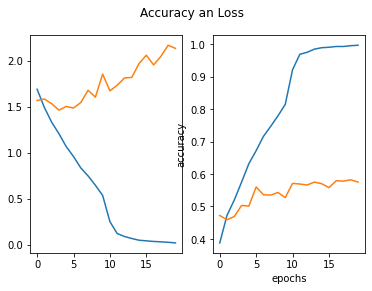
\includegraphics[width = 4in]{../src/acc_plot.png}
\end{figure}
\begin{center}
    \large {Best test accuracy: \textbf{---testAccuracy}} \\
    \large {respective train accuracy: ---trainAccuracy} \\
\end{center}
%------------------------------------- Parameters
\section{Parameters}
\subsection{Net Parameters}

\begin{table}[H]
    \centering
    ---netParameters
\end{table}
    
    
\subsection{Dataset Parameters}
\begin{table}[H]
    \centering
    ---datasetParameters
\end{table}

\subsection{Training Parameters}
\begin{table}[H]
    \centering
    ---trainingParameters
    \end{table}


%------------------------------------- Results
\section{Results}
\subsection{Performance}
\begin{table}[H]
    \centering
        ---performanceTable
\end{table}
\subsection{Confusion Matrix}
\begin{figure}[H]
    \centering
    % \includegraphics[width = 4in]{src/confusion.png}
\end{figure}
\subsection{Stability}
\begin{table}[H]
    \centering
    ---noiseTable
\end{table}  


\subsection{Miss classifications}
\begin{figure}[H]
    \centering
    % \includegraphics[width = 4in]{src/missClassifications.png}
\end{figure}


\end{document}